\newpage
\section{Acquisizione delle informazioni nel telerilevamento}
\subsection{Le Radiazioni elettromagnetiche}
L'acquisizione delle informazioni da remoto su un territorio è possibile attraverso 
l'uso di radiazioni elettromagnetiche (EMR) \cite{OndeEletroMagnetiche}, che vengono emesse o riflesse 
dagli oggetti osservati.
Una radiazione elettromagnetica è una perturbazione di natura simultaneamente 
elettrica e magnetica che si propaga nello spazio e che può trasportare energia.  

% Essa è  lunghezza d’onda 
% $(\lambda)$, frequenza $(f)$ e ampiezza $(A)$. 
% La lunghezza d’onda è la distanza che separa due creste consecutive; la frequenza equivale al numero di picchi
% d’onda che passano in un punto in un intervallo di tempo di un secondo, ed è inversamente
% proporzionale alla lunghezza d’onda; l’ampiezza è la distanza del massimo della cresta dall’asse di
% propagazione dell’onda.

\begin{figure}[H]
    \centering
    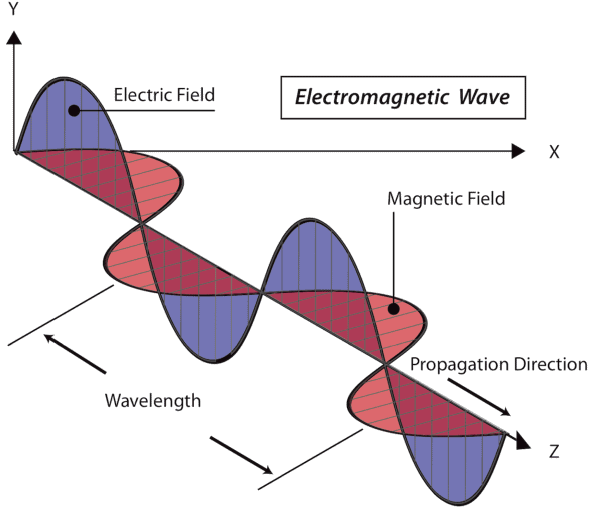
\includegraphics[width=0.44\textwidth]{Immagini/Generiche/OndaElettromagnetica.png}
    \caption{Rappresentazione dell’onda elettromagnetica \cite{Onda_IMG}.}
    \label{fig:onda_elettromagnetica}
\end{figure}

Un’onda elettromagnetica è caratterizzata da tre parametri fondamentali :

\begin{itemize}
    \item \textbf{Lunghezza d’onda $(\lambda)$} la quale esprime la distanza tra due creste d’onda 
    consecutive. La lunghezza d’onda si misura in metri [$m$], o in sottomultipli 
    del metro, come i nanometri ($nm$, $10^{-9}$ metri) o i micrometri ($\mu m$, $10^{-6}$ 
    metri); 

    \item \textbf{Frequenza $(f)$}, cioè il numero dei picchi d’onda che passano in un punto in 
    un certo intervallo di tempo $t$; la frequenza è di solito misurata in hertz [$\text{Hz}$], 
    che è equivalente ad un ciclo al secondo;

    \item \textbf{Ampiezza A}, che è l’altezza di ogni picco d’onda.
\end{itemize}

La frequenza e la lunghezza d’onda sono legate da una relazione, che è definita come:
\begin{equation}
    \lambda = \frac{C}{f}
\end{equation}

dove $C$ è una costante che ha valore $\textit{299.792.458}\ m/s$. Questa costante 
è la velocità della luce e rappresenta la velocità con cui si propaga 
l'onda elettromagnetica attraverso lo spazio. 

\newpage
\subsection{Lo Spettro Elettromagnetico}
La figura (\ref{fig:BandeSpettroElettromagnetico}) rappresenta lo spettro
elettromagnetico (o spettro EM), una distribuzione monodimensionale 
continua dell’energia elettromagnetica, ordinata per lunghezze d’onda $(\lambda)$ crescenti.  
In pratica, lo spettro elettromagnetico è l’insieme di tutte le possibili 
frequenze delle onde elettromagnetiche \cite{spetto_magnetico}.

\begin{figure}[H]
    \centering
    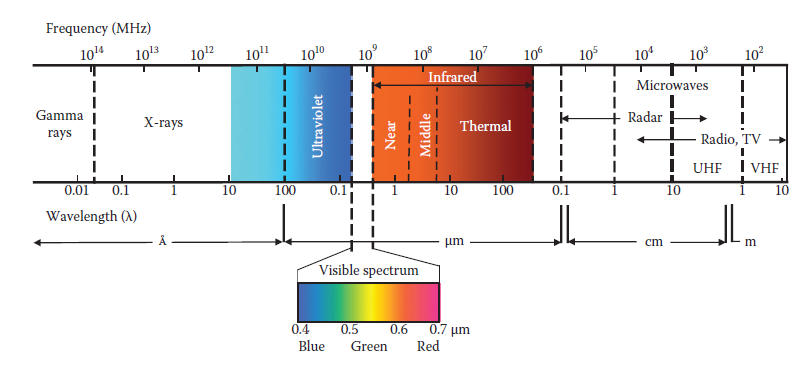
\includegraphics[width=0.95\textwidth]{Immagini/Generiche/BandeSpettroElettromagnetico.png}
    \caption{Bande dello spettro elettromagnetico \cite{SPETTRO_IMG} .}
    \label{fig:BandeSpettroElettromagnetico}
\end{figure}

Come si può osservare, lo spettro è diviso in sette intervalli (anche detti bande),
ciascuna della quali racchiude un insieme di frequenze (o lunghezze d’onda) 
appartenenti alla stessa tipologia di radiazione.

% \begin{figure}[H]
%     \centering
%     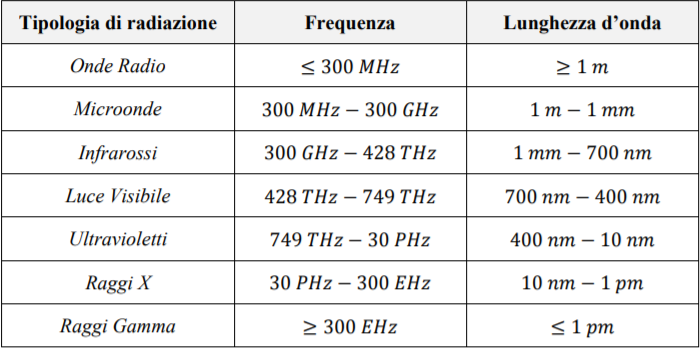
\includegraphics[width=0.65\textwidth]{Immagini/Generiche/Tabella_frequenze.png}
%     \caption{ Classificazione delle radiazioni elettromagnetiche.}
%     \label{fig:Classificazion_radiazioni_elettromagnetiche.}
% \end{figure}

\begin{table}[H]
    \centering
    \begin{tabular}{|p{5cm}|p{5cm}|p{5cm}|}
        \hline
        \textbf{Tipologia di radiazione} & \textbf{Frequenza} & \textbf{Lunghezza d’onda} \\
        \hline
        \textit{Onde Radio} & $\leq 300$ MHz & $\geq 1$ m \\
        \hline
        \textit{Microonde} & $300$ MHz – $300$ GHz & $1$ m – $1$ mm \\
        \hline
        \textit{Infrarossi} & $300$ GHz – $428$ THz & $1$ mm – $700$ nm \\
        \hline
        \textit{Luce Visibile} & $428$ THz – $749$ THz & $700$ nm – $400$ nm \\
        \hline
        \textit{Ultravioletti} & $749$ THz – $30$ PHz & $400$ nm – $10$ nm \\
        \hline
        \textit{Raggi X} & $30$ PHz – $300$ EHz & $10$ nm – $1$ pm \\
        \hline
        \textit{Raggi Gamma} & $\geq 300$ EHz & $\leq 1$ pm \\
        \hline
    \end{tabular}
    \caption{Tabella riassuntiva delle frequenze di ogni tipologia di radiazione.}
\end{table}

Lo spettro del visibile (visible spectrum) è quella parte dello spettro 
elettromagnetico, compresa tra i $400\ nm$ (viola) e $700\ nm$ (rosso), che è percepibile 
all’occhio umano.
% È importante notare come questa sia l’unica parte dello spettro a cui sia 
% possibile associare il concetto di colore.

Tra le diverse regioni spettrali, quelle che vengono principalmente utilizzate 
per l'acquisizione di informazioni su un territorio sono: l'infrarosso (Infrared), 
il visibile (visible) e l'ultravioletto (Ultraviolet). 

% \subsection{Interazioni con l’atmosfera e con la superficie terrestre}
% % La radiazione solare, prima di raggiungere la superficie terrestre percorre 
% % l’atmosfera: in questo passaggio una parte dell’energia è riflessa verso l’alto; 
% % un’altra parte viene invece assorbita e poi riemessa in tutte le direzioni come 
% % radiazione termica; una parte viene diffusa. L’energia elettromagnetica riflessa e 
% % parte di quella diffusa trasporta le informazioni registrate dai radiometri e dai 
% % sensori utilizzati nel telerilevamento.

% Le radiazioni elettromagnetiche posso interagire in diversi 
% modi con l’atmosfera e con la superficie terrestre. 
% Tali interazioni possono essere rilevanti o trascurabili ai fini dei rilievi spettrali, in
% quanto, a seconda del percorso che l’onda deve percorrere prima di essere catturata dal sensore,
% possono influenzare la misurazione del sensore.

% % Le interazioni atmosferiche della radiazione elettromagnetica possono essere 
% % rilevanti o trascurabili ai fini dei rilievi spettrali, a seconda del percorso che l’onda 
% % deve percorrere prima di essere catturata dal sensore. Maggiore è tale percorso, 
% % maggiori sono le influenze atmosferiche sulla radianza registrata dal sensore: se il 
% % sensore è montato su un aereo che vola a bassa quota o se le misure vengono 
% % effettuate a terra, gli effetti dell’atmosfera nella radiazione riflessa sono minimi; al 
% % contrario i sensori montati su satellite ne sono molto influenzati, perché la 
% % radiazione riflessa deve attraversarla completamente prima di raggiungerli.


% L’atmosfera modifica la radiazione in tre modi differenti:
% \begin{itemize}
%     \item Diffusione;
%     \item Assorbimento atmosferico;
%     \item Rifrazione.
% \end{itemize}

% Mentre la superficie terrestre interagisce con la radiazione elettromagnetica
% attraverso processi di:

% \begin{itemize}
%     \item Riflessione;
%     \item Trasmissione;
%     \item Assorbimento terrestre.
% \end{itemize}

% La figura (\ref{fig:interazioni_ondeElettromagnetiche}) mostra un rappresentazione 
% di queste interazioni:

% \begin{figure}[H]
%     \centering
%     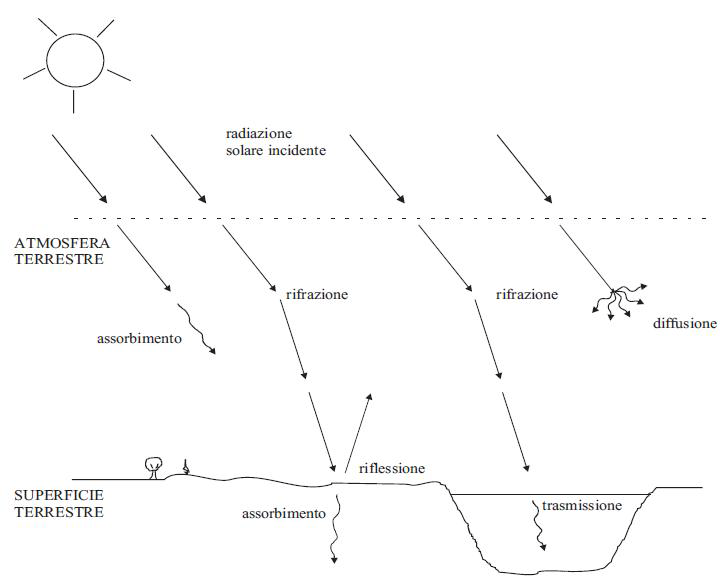
\includegraphics[width=0.70\textwidth]{Immagini/Generiche/interazioni_ondeElettromagnetiche.png}
%     \caption{Interazioni con le onde elettromagnetiche \cite{INTERAZIONI_ONDE}}
%     \label{fig:interazioni_ondeElettromagnetiche}
%     %Figura 2.1: Esempio schematico di un neurone
% \end{figure}

% La \textbf{diffusione} si verifica per interazione con le particelle fini o gassose 
% dell’atmosfera e distribuisce in tutte le direzioni la radiazione intercettata. La 
% diffusione avviene in prevalenza per le radiazioni a lunghezza d’onda più bassa, 
% vale a dire per quelle nel campo del violetto e del blu.

% La \textbf{rifrazione} avviene quando il fascio di luce attraversa due mezzi differenti 
% in grado di trasmettere la radiazione. Nell’atmosfera questo fenomeno avviene al 
% passaggio dei diversi strati atmosferici caratterizzati da umidità e temperature 
% differenti. Tali variazioni influenzano la densità degli strati atmosferici causando 
% una curvatura del raggio che li attraversa. Questo fenomeno è osservabile d’estate
% quando è percepibile un tremolio degli oggetti posti a distanza, dovuto al 
% passaggio della luce vicino a superfici molto calde, come ad esempio il manto 
% stradale. 

% L’\textbf{assorbimento atmosferico} si verifica per l’interazione della radiazione 
% elettromagnetica con i gas presenti nell’atmosfera, quali ozono, ossigeno, anidride 
% carbonica e vapor acqueo. Questi gas assorbono l’energia contenuta nella 
% radiazione luminosa per poi riemetterla sotto forma di energia radiante con 
% lunghezza d’onda maggiore.

% La \textbf{riflessione} avviene quando un raggio luminoso incide su una superficie non 
% trasparente e viene diretto in un’altra direzione. Il tipo di riflessione dipende dalle 
% dimensioni delle irregolarità della superficie: se essa è liscia in 
% relazione alla lunghezza d’onda, si verifica il fenomeno della riflessione speculare 
% in cui tutta la radiazione incidente viene riflessa in un'unica direzione, se la 
% superficie è invece irregolare si comporta come un riflettore isotropo (o diffuso) e 
% la luce viene riflessa in modo diffuso. 

% La \textbf{trasmissione} avviene quando la radiazione passa attraverso un mezzo senza 
% subire una significativa attenuazione.

% L’\textbf{assorbimento terrestre} della radiazione elettromagnetica può avvenire in 
% base alle caratteristiche chimico-fisiche dei corpi che vi si trovano. Ad esempio la 
% vegetazione assorbe gran parte della radiazione incidente della banda del rosso, 
% per poi riemetterla sotto forma di energia termica a lunghezza d’onda maggiore. In 
% natura ogni oggetto ha un comportamento spettrale caratteristico 
% \cite{fenomeni_luce,fenomeni_luce_2,ALL1_REMOTE_SENSING,ALL6_REMOTE_SENSING}. 

\newpage
\subsection{La Radianza e la Riflettanza}
Nel telerilevamento, quello che viene misurato dai sensori è la Radianza e Riflettanza. 
La radianza è definita come la quantità di radiazione elettromagnetica riflessa 
(o trasmessa) per unità di superficie e di angolo solido (angolo nello spazio 
tridimensionale). La radianza rappresenta una grandezza fondamentale nel 
telerilevamento in quanto molto utile per quantificare la luce riflessa da un 
oggetto che viene ricevuta da un sensore rivolto verso di essa. Questa grandezza 
fisica è legata sia alla geometria dell’osservazione, sia alle caratteristiche del 
sensore e permette di descrivere come la radiazione si distribuisce nello spazio
\cite{Radianza, ALL6_REMOTE_SENSING}. 

La radianza è caratterizzata dalla seguente formula: 
\begin{equation}
    L = \frac{P}{A \Omega \cos ({\theta})} \left[\frac{W}{m^2sr}\right]
\end{equation}

dove:
\begin{itemize}
    \item $L$ è la radianza;
    \item $P$ è la potenza in watt;
    \item $\theta$ è l'angolo compreso tra la normale alla superficie e la direzione specificata;
    \item $A$ è la superficie emittente;
    \item $\Omega$ è l'angolo solido.
\end{itemize}

\begin{figure}[H]
    \centering
    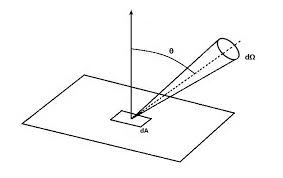
\includegraphics[width=0.40\textwidth]{Immagini/Grafici/radianza.png}
    \caption{Rappresentazione della radianza \cite{RADIANZA_IMG}.}
    \label{fig:Radianza}
    %Figura 2.1: Esempio schematico di un neurone
\end{figure}

La riflettanza invece è il rapporto tra la quantità di radiazione emessa (ovvero 
che colpisce una superficie) e la quantità di radiazione riflessa (o ricevuta) dalla stessa 
ed è quindi un numero puro generalmente minore di uno. 
Questa grandezza è indispensabile per l’individuazione e la discriminazione dei 
campioni oggetto di analisi, in quanto consente di svincolarsi completamente da 
condizioni variabili nel tempo (che influenzano la radianza) al momento 
dell’acquisizione, rendendo confrontabili misure condotte in momenti diversi
\cite{Riflettanza, ALL6_REMOTE_SENSING}. 
La riflettanza può essere espressa come: 

\begin{equation}
    \rho = \frac{\Phi_r}{\Phi_0}
\end{equation}

dove:
\begin{itemize}
    \item $\rho$ è la riflettanza;
    \item $\Phi_r$ il flusso luminoso riflesso;
    \item $\Phi_0$ il flusso luminoso incidente;
\end{itemize}
Ciò che viene direttamente misurato dal sensore è la radianza, per questo è necessaria una corretta 
calibrazione del sensore al fine di ottenere dati confrontabili.



\subsection{Firma spettrale}
Quando la riflettanza o la radianza è calcolata su tutte le frequenze dello spettro, 
si parla allora di \textbf{firma spettrale}. 

%L'imaging multispettrale si basa sulla spettroscopia e sull'ottica.
Ogni oggetto o unità di territorio (roccia, vegetazione…) ha la propria \textbf{firma spettrale} (o impronta digitale spettrale), 
che specifica il modo in cui le lunghezze d'onda della luce vengono assorbite, riflesse o trasmesse attraverso 
quell'oggetto \cite{Firma_spettare}. %Tale proprietà determina il colore nel campo visibile.
% Per esempio, confrontando la firma spettrale di campioni sconosciuti 
% con quella di sostanze note, è possibile identificata la composizione chimica del 
% campione ignoto.

\begin{figure}[H]
    \centering
    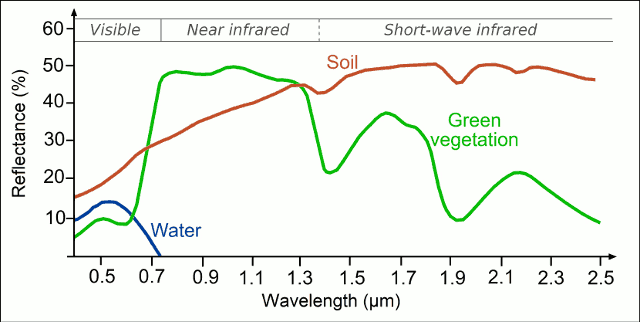
\includegraphics[width=0.70\textwidth]{Immagini/Generiche/spectral_sign.png}
    \caption{Esempi di firme spettrali per acqua, suolo, vegetazione \cite{ALL2_REMOTE_SENSING}.}
    %Figura 2.1: Esempio schematico di un neurone
\end{figure}

Ad esempio i canali utilizzati per la copertura della vegetazione catturano 
l'intensità della luce dal visibile all'infrarosso, consentendo di valutare l'attività fotosintetica e lo stato 
delle piante. I canali per il monitoraggio delle superfici terrestri possono registrare 
l'energia in una gamma più ampia, che comprende gli ultravioletti e le microonde.

\section{Tipologie di sensori}
I sensori possono essere classificati in base a diversi fattori.
Una delle classificazioni più comuni vede i sensori suddivisi in due gruppi: sensori passivi e 
sensori attivi. 
\begin{itemize}
    \item I \textbf{sensori passivi} si limitano a misurare la radiazione elettromagnetica derivata da 
    fonti esterne: ad esempio, l’energia della radiazione solare riflessa dalla superficie 
    terrestre o l’energia direttamente emanata dalla Terra, ovvero la Radianza. 
    Questi sensori sono stati ampiamente utilizzati nel telerilevamento negli ultimi decenni e includono: 
    fotocamere, scanner elettro-ottici e radiometri a microonde.

    \begin{figure}[H]
        \centering
        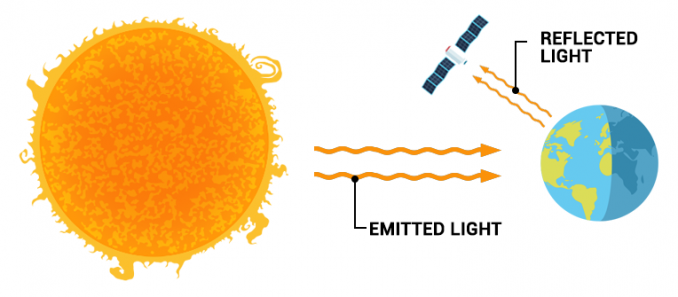
\includegraphics[width=0.65\textwidth]{Immagini/Generiche/Passive-Remote-Sensing.png}
        \caption{Illustrazione funzionamento sensori passivi \cite{GISGeography_RemoteSensing}}
        %Figura 2.1: Esempio schematico di un neurone
    \end{figure}

    \item I \textbf{sensori attivi} sono invece quelli che misurano la radiazione emessa da una fonte 
    di energia incorporata nello strumento stesso e che viene riflessa dalle superfici 
    inquadrate. Ovvero che si basano sul concetto della riflettanza. Questi sono in grado di inviare impulsi e registrare in seguito la loro 
    riflessione per caratterizzare gli oggetti. Queste tipologie di sensori
    sono ad esempio radar o LiDAR.

    \begin{figure}[H]
        \centering
        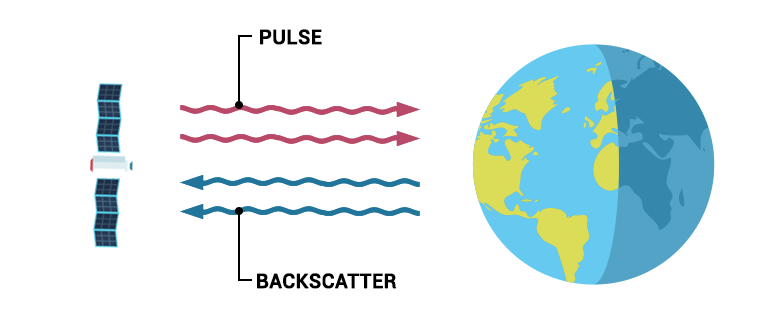
\includegraphics[width=0.65\textwidth]{Immagini/Generiche/Active-Remote-Sensing.png}
        \caption{Illustrazione funzionamento sensori attivi \cite{GISGeography_RemoteSensing}}
        %Figura 2.1: Esempio schematico di un neurone
    \end{figure}

\end{itemize}

I sensori posso essere classificati anche in base al numero di bande che sono in grado di acquisire, i sensori possono essere 
multispettrali o iperspettrali. 

\begin{itemize}
    \item I \textbf{sensori multispettrali} di solito riescono ad acquisire 
    da 3 a 10 bande circa. Le bande che vengono normalmente acquisite sono quelle 
    del visibile, rosso, verde, blu, e quella del vicino infrarosso.

    \item I \textbf{sensori iperspettrali}, invece, misurano l'energia in bande più strette e numerose rispetto ai sensori 
    multispettrali. Le immagini iperspettrali, infatti, possono contenere fino a 200 (o 
    più) bande spettrali. 
\end{itemize}